\documentclass[10pt,a4paper]{article}
\usepackage[utf8]{inputenc}
\usepackage[french]{babel}
\usepackage[T1]{fontenc}
\usepackage{amsmath}
\usepackage{amsfonts}
\usepackage{amssymb}
\usepackage{graphicx}
%%%\usepackage{version}%%%

\title{Resolution de problemes\\ TD}
\date{}
\author{Charles Fallourd}

\begin{document}
\maketitle
\part*{Problèmes de satisfaction de contraintes}

\section*{Le design des Jolioto}


\begin{align*}
X &=& { Rose, Verte, Noire, Blanche }\\
D(PO) &=& D(CP) = { Rose, Verte, Noire }\\
D(CA) &=& { Blanche, Rose, Verte, Noire}\\
D(PC) &=& { Blanche }\\
D(BA) &=& { Verte }\\
D(EJ) &=& {Rose, Verte }\\
\end{align*}

\begin{figure}[H] 
\centering
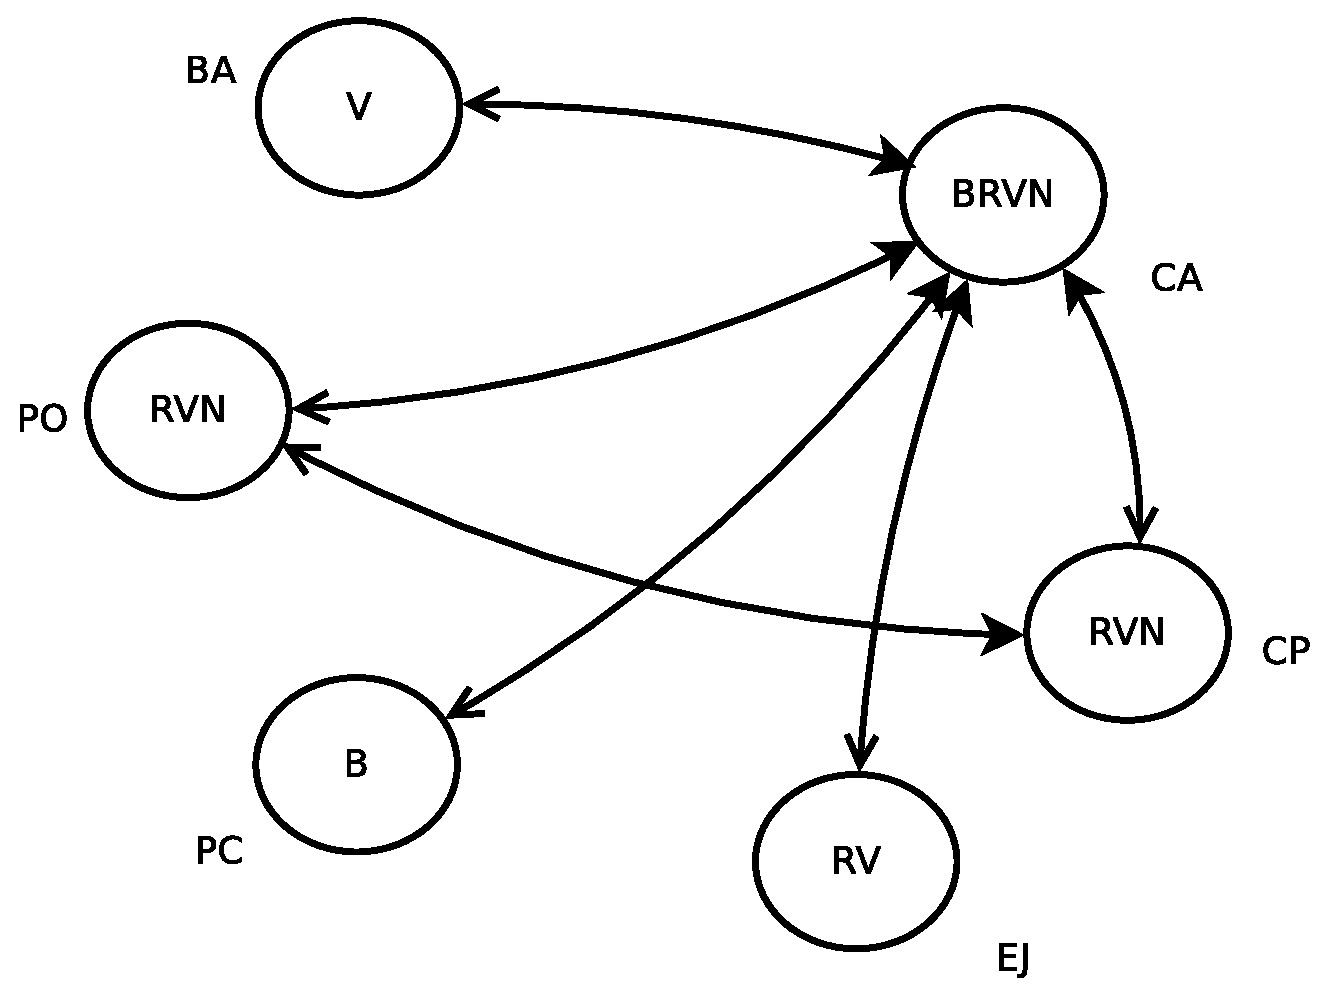
\includegraphics[scale=1.5]{diagramme1.eps}

\end{figure}

\begin{tabular}{ccccccc}
\hline
variables & CA & CP & PO & BA & EJ & PC \\
\hline
Domaines & BRVN & RVN & RVN & V & RV & B \\
\hline
CA $\leftarrow$ B & $\oslash$ (BT) & & & & &\\
\hline
CA $\leftarrow$ R & R & R & $\oslash$ (BT) & & & \\
\hline
CA $\leftarrow$ V & V & V & $\oslash$ (BT) & & & \\
\hline
CA $\leftarrow$ N & N & N & V & RV & B \\
\hline
CP $\leftarrow$ N & N & N & V & RV & B \\
\hline
PO $\leftarrow$ N & N & N & V & RV & B \\
\hline
BA $\leftarrow$ V & N & N & V & RV & B \\
\hline
EJ $\leftarrow$ R & N & N & V & R & B \\
\hline
PC $\leftarrow$ B & N & N & V & R & B \\
\end{tabular}

Deuxième solution : (Backtrack à partir de BA)\\
\begin{tabular}{ccccccc}
\hline
EJ $\leftarrow$ R & N & N & V & R & B \\
\hline
PC $\leftarrow$ B & N & N & V & R & B \\
\end{tabular}
\end{document}